\section{Initial state of Giraf}
%What is the initial state of Giraf
In the beginning of the semester, the only functioning app was the Weekplanner app\cite{AppsStatus2019} hence it is the only app described briefly in this report. In the Weekplanner App, it is possible to make week schedules. In each schedule there is an entry for every day of the week, see \autoref{fig:WeekPlannerPicture}. 

\begin{figure}[h]
        \begin{center}
            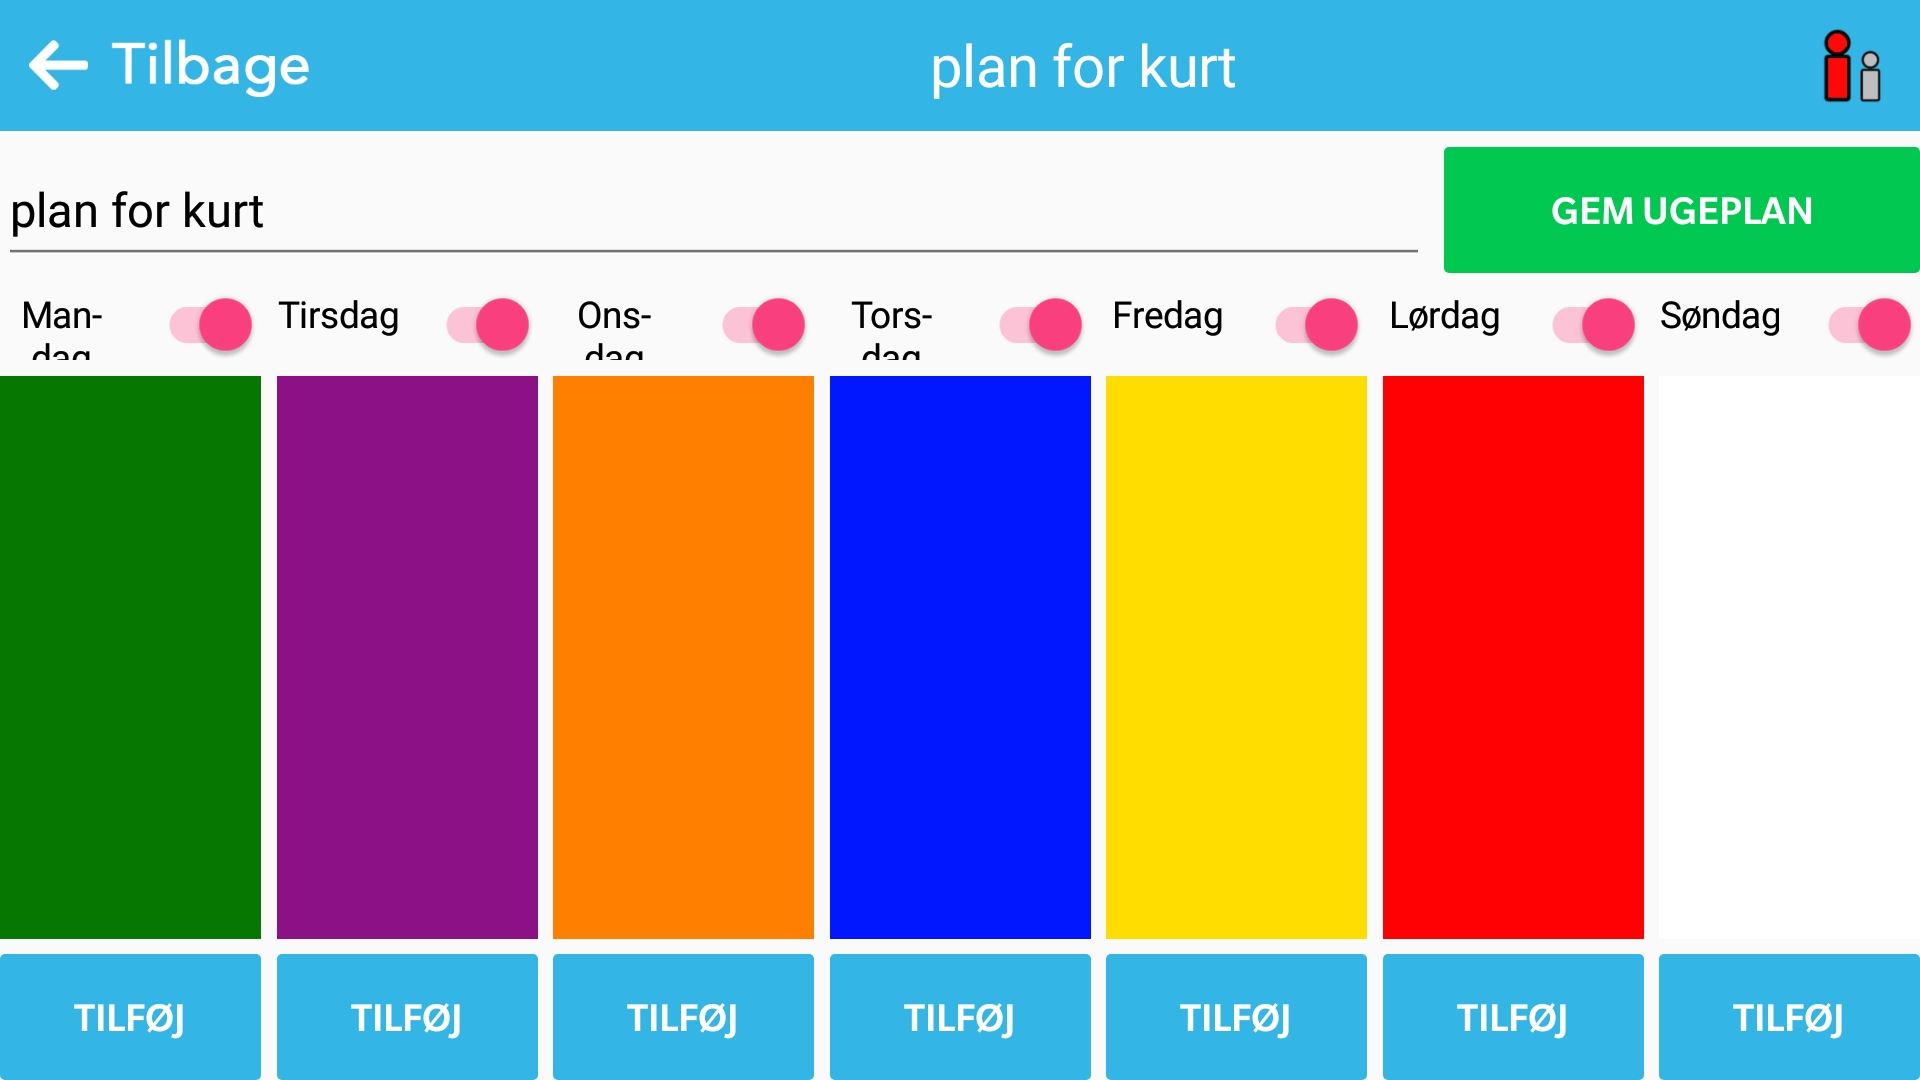
\includegraphics[width=0.95\textwidth]{figures/WeekPlannerPicture}
        \end{center}
        \caption{Weekplanner state at the start of 2019}
        \label{fig:WeekPlannerPicture}
\end{figure}

On each day a series of pictograms can be placed. These pictograms symbolizes an activity that has to be performed that day, the activities will then be performed from the top down. 

%This way of representing activities is a well known approach for showing autistic people what will happen, and is often done using physical pictograms representing every activities. This can however be difficult when a new kind of activity is needed, because a new instance have to be found and cut out every time\cite{AutistTeacher}. In a digital solution, there only need to be constructed a new pictogram, and this can be used as much as needed, no cutting required. 
%The other apps are no longer used, and will therefore not be described.
 %\end{comment}
%- Standards
%- Strengths and weaknesses 